\subsection{Tworzenie nowych typów danych}

Funkcjonalność tworzenia nowych typów danych nie wyróżnia przygotowanego systemu
od systemów CMS dostępnych na rynku. Jest zaimplementowana, jako lista
formularzy. Każdy formularz odpowiada jednej kolumnie w nowo utworzonej tabeli.
Administrator może dodawać nowy formularz, lub kasować już istniejący.

Pojedyńczy formularz zawiera następujące elementy:

\begin{itemize}

    \item Pole tekstowe, gdzie administrator podaje nazwę kolumny.

    \item Menu rozwijane pozwalające na wybór typu kolumny.

    \item Pole wyboru, które pozwala określić administratorowi, czy kolumna może
    zawierać wartości \verb|null|.

    \item Pole wyboru, które pozwala określić czy kolumna posiada wartość
    domyślną wraz z polem tekstowym, które pojawia się, gdy administrator
    oznaczy kolumnę jako posiadającą wartość domyślną, gdzie należy podać
    wartość domyślną.

\end{itemize}

Interfejs tworzenia nowych typów danych jest pokazany na rysunku \ref{tableCreationFigure}.

\begin{figure}[h]
    \centering
    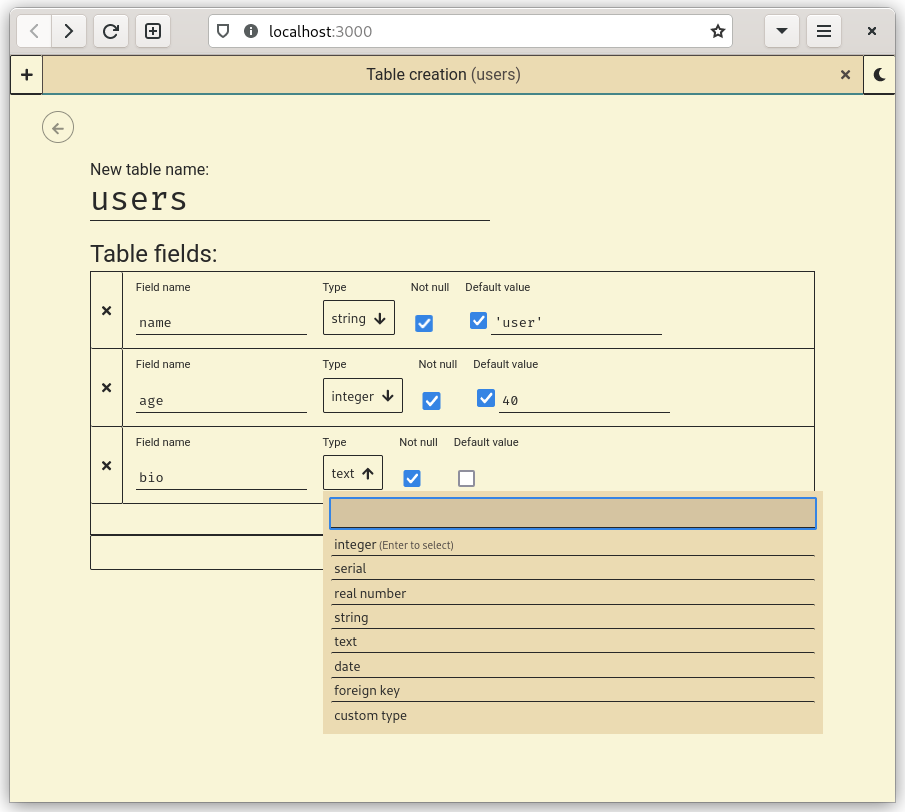
\includegraphics[width=0.8\textwidth]{./img/table_creation.png}
    \caption{Interfejs tworzenia nowego typu danych}
    \label{tableCreationFigure}
\end{figure}

\subsection{Zarządzanie danymi}
